% !TeX spellcheck = es_ES
% !TeX encoding = ISO-8859-1

Una vez establecido el hardware y realizado el dise�o del software necesario para implementar la aplicaci�n en el microcontrolador se realiz� una serie de pruebas para constatar la correcta implementaci�n del sistema.

\section{Resultados de la interfaz gr�fica}

Para realizar las pruebas del sistema que se presentan a continuaci�n se debi� configurar cada uno de los nodos utilizando la interfaz gr�fica implementada en el modo de configuraci�n. A continuaci�n se ilustran las distintas pantallas implementadas en ellas:

\begin{figure}[H]
	\centering
	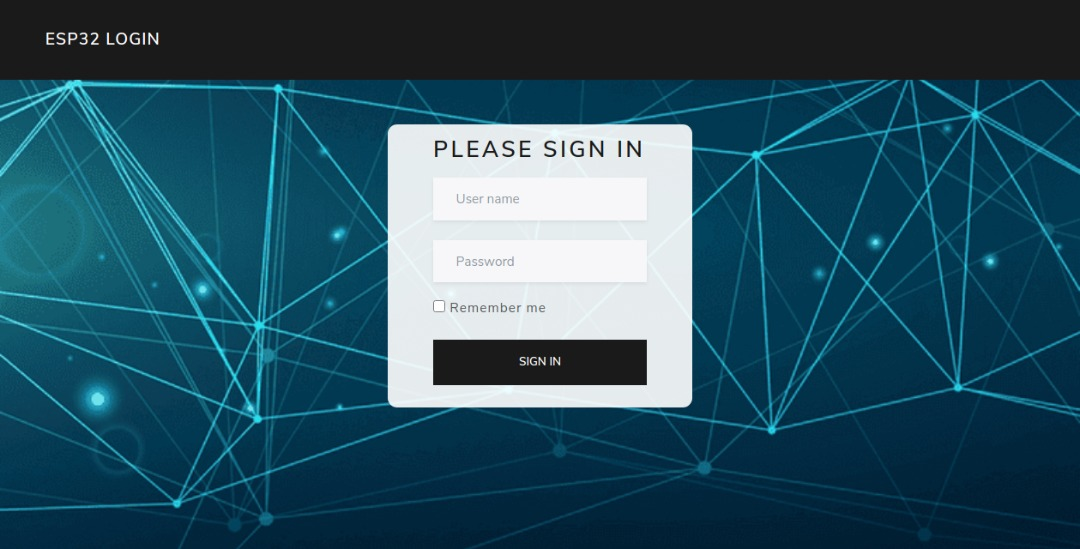
\includegraphics[width=0.9\linewidth]{img/Login}
	\caption{Vista de la pantalla de inicio de sesi�n del usuario.}
	\label{fig:login}
\end{figure}

\begin{figure}[H]
	\centering
	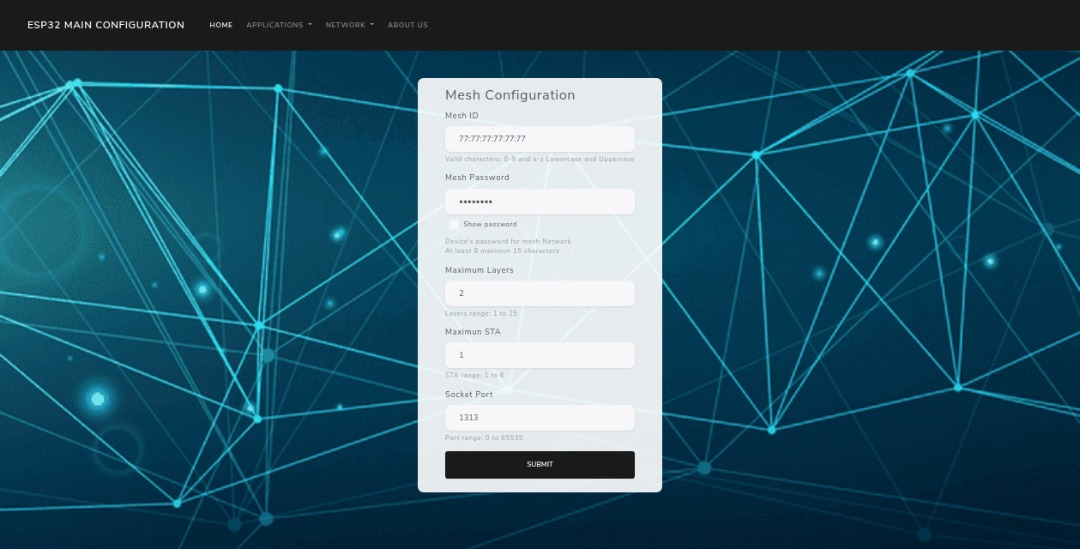
\includegraphics[width=0.9\linewidth]{img/FormMesh}
	\caption{Vista de la pantalla del formulario de par�metros de la red mallada.}
	\label{fig:formmesh}
\end{figure}


\begin{figure}[H]
	\centering
	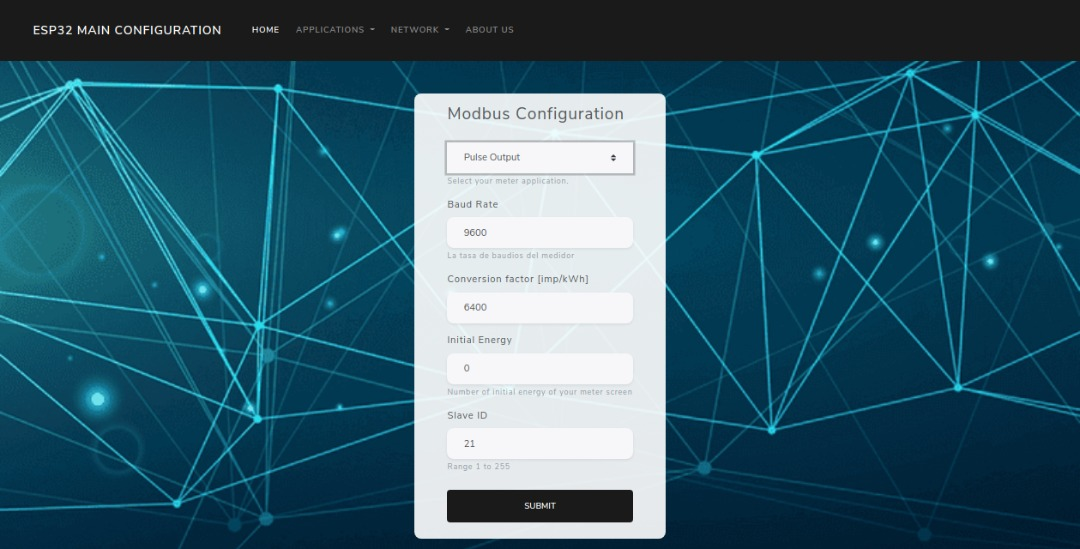
\includegraphics[width=0.9\linewidth]{img/FormModbus}
	\caption{Vista de la pantalla de formulario de par�metros seriales.}
	\label{fig:formmodbus}
\end{figure}

\begin{figure}[H]
	\centering
	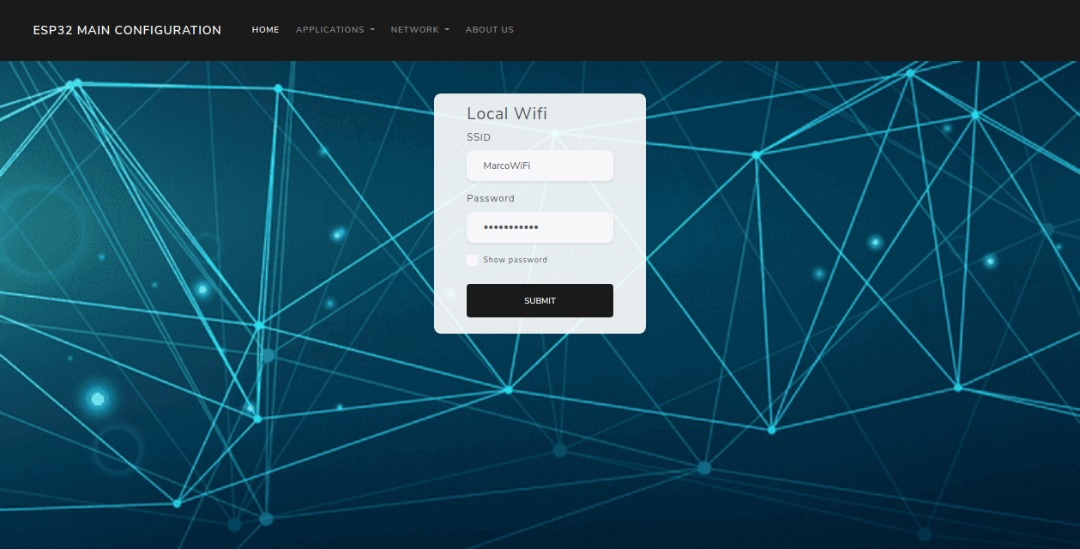
\includegraphics[width=0.9\linewidth]{img/LocWifijpg}
	\caption{Vista de la pantalla de par�metros de red local}
	\label{fig:locwifijpg}
\end{figure}

\begin{figure}[H]
	\centering
	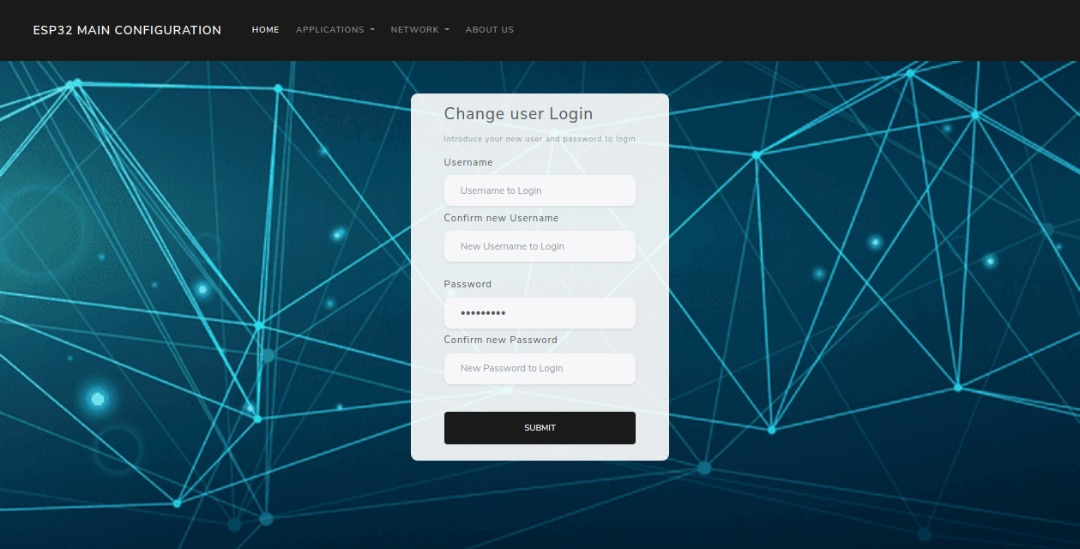
\includegraphics[width=0.9\linewidth]{img/UserLog}
	\caption{Vista de la pantalla para modificar los par�metros de acceso del usuario.}
	\label{fig:userlog}
\end{figure}


\section{Prueba de funcionamiento del sistema}

\subsection{Extracci�n de datos del nodo contador de pulsos}

\begin{table}[H]
	\centering
	\caption{Registro de mensajes del maestro sobre la comunicaci�n con el esclavo de pulsos.}
	\label{Tab:Master2Pulse}
	\medskip
	\begin{tabular}{l|lllr}
		\toprule
		\multicolumn{5}{c}{Nodo maestro} \\
		\#&Enviados& Recibidos& Tiempo de prueba [s]& Errores detectados\\
		\midrule
		1&1500  & 1499  & 2223,801 & 13   \\
		2&1500 & 1499  & 2226,643 & 16   \\
		3&1500& 1500 & 2226,970 & 15\\
		\bottomrule
	\end{tabular}
\end{table}

\begin{table}[H]
	\centering
	\caption{Registro de mensajes del nodo contador de pulsos sobre la comunicaci�n con el maestro.}
	\label{Tab:Pulse2Master}
	\medskip
	\begin{tabular}{l|lllr}
		\toprule
		\multicolumn{5}{c}{Nodo contador de pulsos} \\
		 \# & Recibidos & Enviados & Tiempo de prueba [s] & Errores detectados \\
		\midrule
		1&1499 & 1499&2223,801 & -\\	
		2&1499 & 1499&2226,643 & -\\
		3&1499 & 1500&2226,970 & -\\
		\bottomrule
	\end{tabular}
\end{table}

\subsection{Extracci�n de datos del nodo RS485}


\begin{table}[H]
	\centering
	\caption{Registro de mensajes del maestro sobre la comunicaci�n con el nodo serial rs485.}
	\label{Tab:Master2Serial}
	\medskip
	\begin{tabular}{l|lllr}
		\toprule
		\multicolumn{5}{c}{Nodo maestro} \\
		\#&Enviados& Recibidos& Tiempo de prueba [s]& Errores detectados\\
		\midrule
		1&1500   & 1481  & 2761,411 & 67   \\
		2&1500  & 1481  & 2761,803 & 67  \\
		3&1500 & 1480 & 2758,267 & 65\\
		\bottomrule
	\end{tabular}
\end{table}

\begin{table}[H]
	\centering
	\caption{Registro de mensajes del nodo serial rs485 sobre la comunicaci�n con el maestro.}
	\label{Tab:Serial2Master}
	\medskip
	\begin{tabular}{l|lllr}
		\toprule
		\multicolumn{5}{c}{Nodo serial RS485} \\
		\# & Recibidos & Enviados & Tiempo de prueba [s] & Errores detectados \\
		\midrule
		1&1498  & 1481 &2761,411 & -\\	
		2&1498  & 1481 &2761,803 & -\\
		3&1498 & 1480 &2758,267 & -\\
		\bottomrule
	\end{tabular}
\end{table}

\section{Prueba de reestablecimiento del sistema}
\subsection{Para el nodo central}
\begin{table}[H]
	\centering
	\caption{Tiempo de recuperaci�n de la red cuando es desconectado el nodo central.}
	\label{Tab:healingMasterNode}
	\medskip
	\begin{tabular}{lr}
		\toprule
		\# & Tiempo de recuperaci�n [ms] \\
		\midrule
		1&25541 \\
		2&24598 \\
		3&25720 \\
		4&25231 \\
		5&24896 \\
		\bottomrule
	\end{tabular}
\end{table}

\subsection{Para cualquier otro nodo}
\begin{table}[H]
	\centering
	\caption{Tiempo de recuperaci�n de la red cuando es desconectado un nodo, exceptuando el nodo central.}
	\label{Tab:healingAnyNode}
	\medskip
	\begin{tabular}{lr}
		\toprule
		\# & Tiempo de recuperaci�n [ms] \\
		\midrule
		1&17776 \\
		2&18163 \\
		3&17142 \\
		4&17964 \\
		5&18162 \\
		6&18254 \\
		7&18422 \\
		8&17968 \\
		9&17566 \\
		10&17001 \\
		\bottomrule
	\end{tabular}
\end{table}
